An important background for any analysis with jets and large \MET is
the production of $Z$ bosons in association with jets, where the $Z$
boson decays to neutrinos.  In this section the estimation of this background
is discussed.  
%The prediction method is the same as the one used in the 13\TeV
%stop analysis from 2015 detailed in Refs.~\cite{CMS-PAS-SUS-16-007} and \cite{2015stopAN}.

Ideally, we would like to use a data driven approach based on
$Z$+jets events where the $Z$ boson decays to a
muon pair. The kinematics of these events are indistinguishable from the
kinematics of events where $Z$ decays to neutrinos.
The behavior under the search region selection and the characteristics
of the distributions of physics observables for both decays, including the minimum
\HT and \MET requirements or the number of b-tagged jets, would be
preserved.
This strategy gives a reliable background estimation, however it suffers from
having a low number of events, which is due in part to the small branching ratio for $Z \rightarrow \mu \mu$
as well as the b-tagging and other kinematic requirements placed on the control
region events.

To improve on the large statistical uncertainties that would occur when using the
above method, a method incorporating data-validated MC is used instead.
In this multistage process the final estimate is taken from the
$Z \rightarrow \nu \nu$ MC, which is corrected for
data/MC differences observed in a control region with loosened selection criteria.

The central value of the $Z \rightarrow \nu \nu$ background prediction
for each search bin $B$ can be written as
\begin{equation}
\widehat{N}_B = R_\textrm{norm} \cdot \sum_{\textrm{events}\in B} S_{DY}(N_\textrm{jet}) w_\textrm{MC}
\label{eq:zinv_pred}
\end{equation}
, with $\widehat{N}_B$ the predicted number of $Z \rightarrow \nu \nu$
background events in search bin $B$, and $w_\textrm{MC}$ the standard MC event
weight including the assumed $Z \rightarrow \nu \nu$ cross section, the data
luminosity, the b tag scale factors,
and the measured trigger efficiency.
Each MC event is corrected using two additional scale factors. The first, $R_\textrm{norm}$,
is an overall normalization factor for the $Z \rightarrow \nu \nu$ simulation
that is derived in a tight control region in data.
This tight control region has the same selection as the search region, apart from
the requirement that there be two muons (treated as if they were neutrinos) and
that events with any b-tagged jet multiplicity are allowed, so it is a very
good proxy for the signal region.
The second scale factor, $S_{DY}$, depends on the number of jets $(N_\textrm{jet})$
in the event and is derived in a loose control region in which the signal region
requirements on \MET, \MTTwo and the number of top-tagged jets in the event are
relaxed.
The scale factor is derived separately for events with 0 and ${\geq}1$ b-tagged
jets. 
It corrects both the observed mismodelling of the jet multiplicity distribution
in the simulation and the difference in normalization between data and simulation
in this loose region.

This corrected MC estimate is further validated, and systematic
uncertainties are assigned where appropriate.
A first sanity check is to validate the $DY\rightarrow \mu \mu$ MC against
the $Z \rightarrow \nu \nu$ MC.  Any expected differences due to generator
discrepancies, acceptance, and efficiency are corrected for.
This is an important step for the overall validation of the method because it relies on
the usage of dimuon events in data to do the various cross checks and derive scale factors.
These scale factors are eventually applied to $Z \rightarrow \nu \nu$ MC events, hence
the need for a good match between $DY\rightarrow \mu \mu$ and $Z \rightarrow \nu \nu$ MC.
A second layer of validation is to use the loose control region, for which a reasonable
number of events are available in data, to check the shape agreement between data
and the simulated distributions.
Any disagreements will be incorporated as a systematic uncertainty in the prediction.
Finally, we also need to check the data/MC agreement in the loose region, where the shape
systematics are assessed, versus the data/MC agreement in the tight region, which is the
proxy for the region we want to predict.


The $Z \rightarrow \nu \nu$ background predictions for each search bin,
including the statistical and systematic uncertainties,
are shown in Fig.~\ref{fig:Zinv_prediction}

\begin{figure}[htbp]
\begin{center}
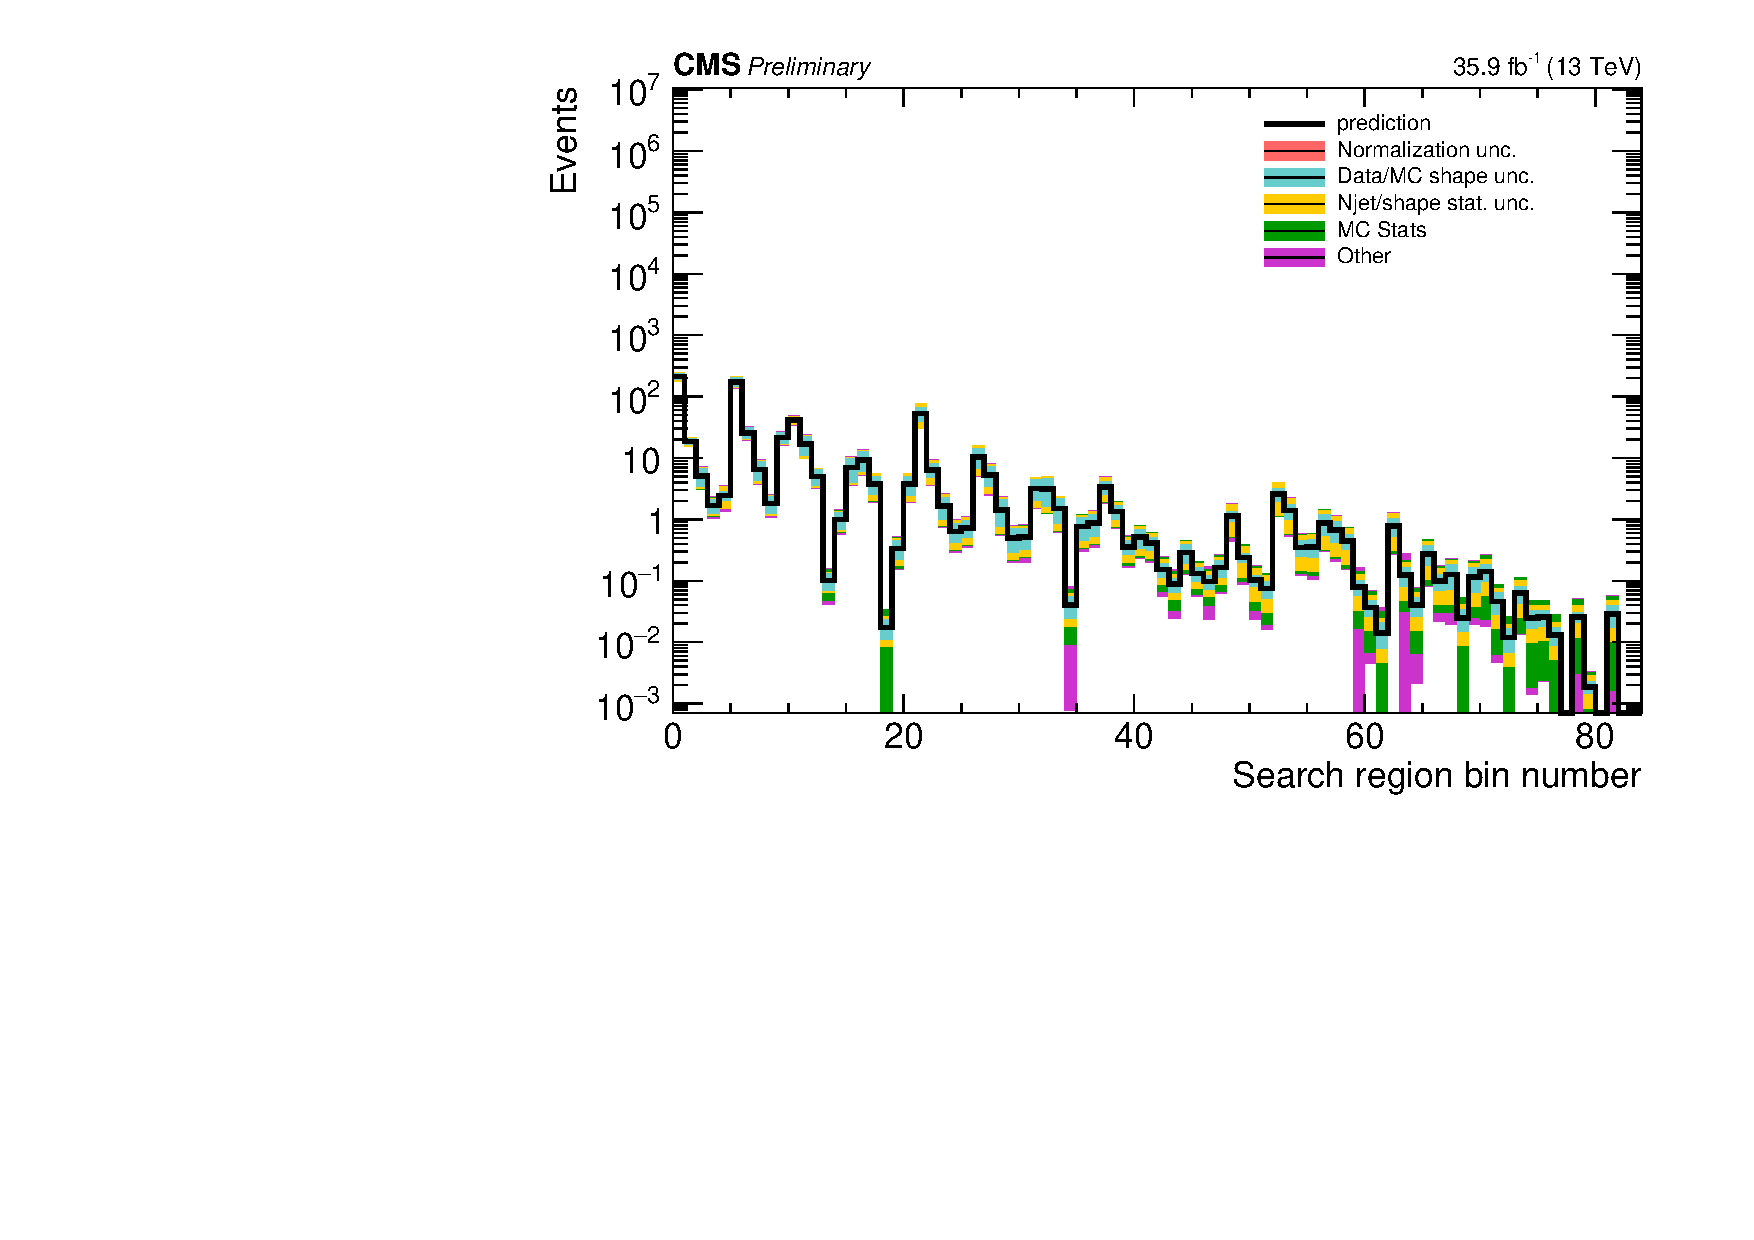
\includegraphics[width=\textwidth]{sections/mc4/Backgrounds/ZInv/figures/moneyplot.pdf}
\end{center}
\caption{$Z\rightarrow\nu\nu$ background prediction for all search bins, including the breakdown of the various uncertainties.}
\label{fig:Zinv_prediction}
\end{figure}

